\subsection*{2. Schritt: Singulärwert-Zerlegung}

Wir führen zunächst eine Singulärwert-Zerlegung von $A_0$ durch.

\begin{align*}
    \tilde V \Sigma \tilde W^\ast = A_0 \in \C^{N \times j},
    \quad
    \tilde V \in \U_N(\C),
    \quad
    \tilde W \in \U_j(\C),
    \quad
    \Sigma_{l, k} = \sigma_l \delta_{l, k},
    \quad
    l = 1, \dots, N,
    \quad
    k = 1, \dots, j
\end{align*}

Nun haben wir angenommen, dass $V, W \in \C^{N \times J}$ vollen Rang $J$ haben und $\hat V \in \C^{N \times j}$ vollen Rang $j$ hat.
Es ist also plausibel, dass $A_0 = V W^\ast \hat V \in \C^{N \times j}$ Rang $J$ hat.
Das wird durch Abbildung \ref{fig:rang_1} illustriert.

\begin{figure}[!ht]
    \centering
    \begin{tikzpicture}[scale = 0.5]

        \begin{scope}
            
            \draw (0,  0) rectangle (2,  6);
            \draw (6,  0) rectangle (8,  6);
            \draw (12, 0) rectangle (14, 6);
            \draw (18, 0) rectangle (20, 6);
    
            \draw (0, 1) -- (2, 1);
            \draw (0, 5) -- (2, 5);
    
            \draw (2, 1) -- (6, 0);
            \draw (2, 5) -- (6, 6);
    
            \draw [dotted] (2, 1) -- (6, 1);
            \draw [dotted] (2, 5) -- (6, 5);
    
            \draw [dotted] (6, 1) -- (8, 1);
            \draw [dotted] (6, 5) -- (8, 5);
    
            \draw (8, 0) -- (12, 2);
            \draw (8, 6) -- (12, 4);
    
            \draw [dotted] (8, 1) -- (12, 2);
            \draw [dotted] (8, 5) -- (12, 4);
    
            \draw (12, 2) -- (14, 2);
            \draw (12, 4) -- (14, 4);
    
            \draw (14, 2) -- (18, 0);
            \draw (14, 4) -- (18, 6);
    
            \draw [dotted] (14, 2) -- (18, 2);
            \draw [dotted] (14, 4) -- (18, 4);
    
            \draw [dotted] (18, 2) -- (20, 2);
            \draw [dotted] (18, 4) -- (20, 4);

        \end{scope}    

        \begin{scope}[yshift = 7 cm]
            
            \draw (1,  0) node {$\C^j$};
            \draw (7,  0) node {$\C^N$};
            \draw (13, 0) node {$\C^J$};
            \draw (19, 0) node {$\C^N$};
    
            \draw (4,  0) node {$\xrightarrow[\text{injektiv}] {\hat V}$};
            \draw (10, 0) node {$\xrightarrow[\text{surjektiv}]{W^\ast}$};
            \draw (16, 0) node {$\xrightarrow[\text{injektiv}] {V}     $};

        \end{scope}

    \end{tikzpicture}
    \caption{}
    \label{fig:rang_1}
\end{figure}

Matrizen haben genau dann denselben Rang, wenn sie äquivalent sind.

\begin{align*}
    \begin{pmatrix}
        \diag(\sigma_1, \dots, \sigma_J, \dots, \sigma_j) \\
        0_{(N - j) \times j}
    \end{pmatrix}
    =
    \Sigma
    \equiv
    \tilde V \Sigma \tilde W^\ast
    =
    A_0
    \equiv
    \begin{pmatrix}
        I_J \enspace 0_{J \times (j - J)} \\ 0_{(N - J) \times j}
    \end{pmatrix}
\end{align*}

Damit verschwinden die letzten Singulärwerte $\sigma_{J+1} = \cdots = \sigma_j = 0$.
Somit können wir statt der vollen Singulärwert-Zerlegung (indiziert mit \Quote{full}) eine reduzierte (indiziert mit \Quote{reduced}) verwenden.

\begin{align*}
    A_0
    =
    \tilde V_\mathrm{full} \Sigma_\mathrm{full} \tilde W_\mathrm{full}^\ast
    =
    \begin{pmatrix}
        \tilde V_\mathrm{reduced} & \ast
    \end{pmatrix}
    \begin{pmatrix}
        \Sigma_\mathrm{reduced} & 0_{J \times (j - J)}       \\
        0_{(N - J) \times J}    & 0_{(N - J) \times (j - J)}
    \end{pmatrix}
    \begin{pmatrix}
        \tilde W_\mathrm{reduced}^\ast \\ \ast
    \end{pmatrix}
    =
    \tilde V_\mathrm{reduced} \Sigma_\mathrm{reduced} \tilde W_\mathrm{reduced}^\ast
\end{align*}

$\tilde V_\mathrm{full} \in \U_N(\C)$ und $\tilde W_\mathrm{full} \in \U_j(\C)$ sind ja unitär, d.h. ihre Adjungierten sind ihre Inversen.

\begin{align*}
    & \implies
    I_{N \times N}
    =
    \tilde V_\mathrm{full}^\ast \tilde V_\mathrm{full}
    =
    \begin{pmatrix}
        \tilde V_\mathrm{reduced}^\ast \\ \ast
    \end{pmatrix}
    \begin{pmatrix}
        \tilde V_\mathrm{reduced} & \ast
    \end{pmatrix}
    =
    \begin{pmatrix}
        \tilde V_\mathrm{reduced}^\ast \tilde V_\mathrm{reduced} & \ast \\
        \ast                                                     & \ast
    \end{pmatrix}, \\
    & \implies
    I_{j \times j}
    =
    \tilde W_\mathrm{full}^\ast \tilde W_\mathrm{full}
    =
    \begin{pmatrix}
        \tilde W_\mathrm{reduced}^\ast \\ \ast
    \end{pmatrix}
    \begin{pmatrix}
        \tilde W_\mathrm{reduced} & \ast
    \end{pmatrix}
    =
    \begin{pmatrix}
        \tilde W_\mathrm{reduced}^\ast \tilde W_\mathrm{reduced} & \ast \\
        \ast                                                     & \ast
    \end{pmatrix}
\end{align*}

Wir vereinbaren, ab sofort nur noch die reduzierte Singulärwert-Zerlegung zu verwenden und den Index wegzulassen.
Insgesamt erhalten wir also folgende Tatsachen über unsere reduzierte Singulärwert-Zerlegung.

\begin{align} \label{eq:singulärwert_zerlegung}
    A_0 = \tilde V \Sigma \tilde W^\ast,
    \quad
    \tilde V^\ast \tilde V
    =
    \tilde W^\ast \tilde W
    =
    I_{J \times J},
    \quad
    \Sigma = \diag(\sigma_1, \dots, \sigma_J) \in \C^{J \times J},
    \quad
    \tilde V \in \C^{N \times J},
    \quad
    \tilde W \in \C^{j \times J}
\end{align}

$\tilde V \in \C^{N \times J}$ hat, als Teil-Matrix einer unitären, vollen Rang $J$.
Es ist also plausibel, dass $S := \tilde V^\ast V \in \C^{J \times J}$ Rang $J$ hat, also $\in \GL_J(\C)$, d.h. invertierbar ist.
Das wird durch Abbildung \ref{fig:rang_2} illustriert.

\begin{figure}[H]
    \centering
    \begin{tikzpicture}[scale = 0.5]

        \begin{scope}
            
            \draw (0,  0) rectangle (2,  6);
            \draw (6,  0) rectangle (8,  6);
            \draw (12, 0) rectangle (14, 6);
    
            \draw (0, 2) -- (2, 2);
            \draw (0, 4) -- (2, 4);
    
            \draw (2, 2) -- (6, 0);
            \draw (2, 4) -- (6, 6);
    
            \draw [dotted] (2, 2) -- (6, 2);
            \draw [dotted] (2, 4) -- (6, 4);

            \draw [dotted] (6, 2) -- (8, 2);
            \draw [dotted] (6, 4) -- (8, 4);

            \draw (8, 0) -- (12, 2);
            \draw (8, 6) -- (12, 4);

            \draw [dotted] (8, 2) -- (12, 2);
            \draw [dotted] (8, 4) -- (12, 4);

            \draw (12, 2) -- (14, 2);
            \draw (12, 4) -- (14, 4);

        \end{scope}    

        \begin{scope}[yshift = 7 cm]

            \draw (1,  0) node {$\C^J$};
            \draw (7,  0) node {$\C^N$};
            \draw (13, 0) node {$\C^J$};

            \draw (4,  0) node {$\xrightarrow[\text{injektiv}]{V}$};
            \draw (10, 0) node {$\xrightarrow[\text{surjektiv}]{\tilde V^\ast}$};

        \end{scope}    

    \end{tikzpicture}
    \caption{}
    \label{fig:rang_2}
\end{figure}

In den folgenden Gleichungsketten wird bei \Quote{!} die jeweils vorgerige eingesetzt.

\begin{align*}
    & \implies
    \Sigma \tilde W^\ast
    \stackrel
    {
        \eqref{eq:singulärwert_zerlegung}
    }{=}
    \tilde V^\ast \tilde V \Sigma \tilde W^\ast
    \stackrel
    {
        \eqref{eq:singulärwert_zerlegung}
    }{=}
    \tilde V^\ast A_0
    \stackrel
    {
        \eqref{eq:integral_matrizen_resultat}
    }{=}
    \tilde V^\ast V W^\ast \hat V
    =
    S W^\ast \hat V \\
    & \implies
    A_1
    \stackrel
    {
        \eqref{eq:integral_matrizen_resultat}
    }{=}
    V D W^\ast \hat V
    \stackrel{!}{=}
    V D S^{-1} \Sigma \tilde W^\ast \\
    & \implies
    \tilde V^\ast A_1 \tilde W \Sigma^{-1}
    \stackrel{!}{=}
    \tilde V^\ast V D S^{-1} \Sigma \tilde W^\ast \tilde W \Sigma^{-1}
    =
    S D S^{-1}
    \approx
    D
\end{align*}

Somit ist die Diagonalmatrix $D$, welche ja die gesuchten Eigenwerte $\lambda_1, \dots, \lambda_k$ von $A$ enthält, ähnlich zur Matrix $\tilde V^\ast A_1 \tilde W \Sigma^{-1}$.
Ähnliche Matrizen haben dieselben Eigenwerte.
